\documentclass[../main/main.tex]{subfiles}


\begin{document}

\section{April 16th, 2019}
\subsection{Multiway Cut Problem}
\begin{itemize}
	\item Given an undirected graph $G=(V,E)$, with costs $c_e\ge 0$ for all edges $e\in E$ and $k$ distinguished vertices $s_1, s_2, \ldots,s_k$ 
	\item Remove a minimum cost set of edges $F$ such that no pair of distinguished vertices are in the same connected components of $(V,E-F)$.
\end{itemize}
\begin{remark}
	For $k=2$, we can reduce this problem into the min $s-t$ problem, by duplicating all undirected edges to get a directed graph. As such for $k=2$, there is a polynomial time solution that can solve this problem exactly. However, for $k\ge 3$, this problem is NP-Complete.
\end{remark}

Application in distributed computing: 
\begin{itemize}
	\item Vertices represent ``Objects''.
	\item $c_e$ represents amount of communication between objects.
	\item We need to place the ``Objects'' in $k$ different machines with a special object $s_i$ which needs to be on machine $i$.
	\item Goal is to partition all the objects onto the $k$ machines so as to minimize the cost of communication.
\end{itemize}
\subsection{2-Approximation Algorithm}
\begin{figure}[h!]
	\centering
	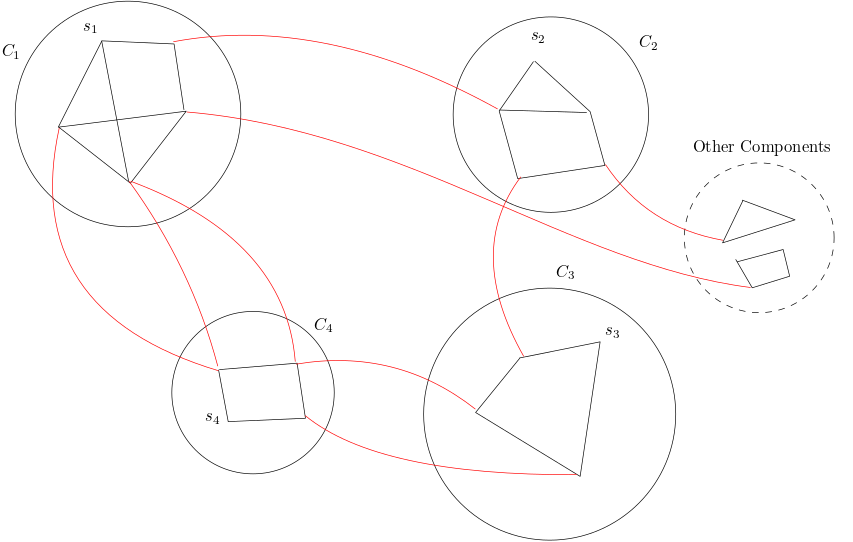
\includegraphics[width=0.8\textwidth]{4-16-mw-e}
	\caption{$F$ is the set of red lines.}
\end{figure}
\begin{itemize}
	\item Define $F_i=\delta(C_i)$ to be the edges in the cut $(C_i, \overline{C_i})$.
	\item $F:$ feasible solution for the multiway cut.
	\item Note that $F_i$ is a cut separating $s_i$ from all the other distinguished vertices. Call $F_i$ an \vocab{isolating} cut as it isolates $s_i$ from all the other distinguished vertices. As such: \[
	F=\bigcup\limits_{i} F_i
	,\] and \[
	\sum_{i} Cost(F_i) \le 2\ Cost(F)
.\] This is because each edge is counted for at most twice (note that edges to ``Other Components'' are only counted once.
\item Note that these above properties apply to any feasible solution $F$, in particular the optimal solution.
\end{itemize}
\begin{remark}	Let  $F_i$ be the minimum isolating cut for $s_i$ (assuming this can be found in polynomial time). $F=\bigcup\limits_{i} F_i$ is the output of our algorithm. Note that  \[
		Cost(F)\le \sum Cost(F_i) \le  \sum Cost(F^*_i)\le 2\ Cost(F^*)
	.\] Now we just need to find the minimum isolating cut.
\end{remark}
\begin{figure}[h!]
	\centering
	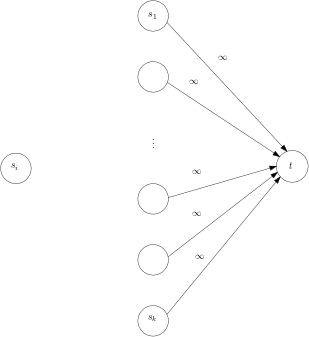
\includegraphics[width=0.4\textwidth]{4-16-mw-cut}
	\caption{$F_i$ can be solved exactly using the $s-t$ min cut in poly-time}
	\label{fig:4-16-mw-cut}
\end{figure}
\begin{remark}
	Note that we can drop the most expensive isolating cut, as if all of the others are isolated, then the last one must be. This will improve our solution by $\left( 1-\frac{1}{k} \right) $, since the most expensive isolating cut must have cost greater or equal to $\frac{1}{k}\ Cost(F^*)$. \\
	
	This means that the new approximation ratio is $2\left( 1-\frac{1}{k} \right) $, which means that $k=3$ has approximation ratio  $\frac{4}{3}$, $k=4\implies \frac{3}{2}$, with $k\to \infty \implies 2$. \\
	
	We will now find an approximation algorithm with approximation factor 1.5.
\end{remark}
\subsection{1.5-Approximation Algorithm}
Reformulation of the problem:
\begin{itemize}
	\item Partition the set of vertices into sets $C_i$ such that $s_i\in C_i$ for all $i$ and such that the cost of \[
			F=\bigcup\limits_{i} \delta(C_i) \text{ is minimized}
		,\] where $\delta(C_i)$ is the set of edges in the cut  $\left( C_i, \overline{C_i} \right) $.
	\item Note that this means that the vertices in the ``Other Components'' can be placed in any group $C_i$.
	\item For each vertex $u\in V$, introduce $k$ different variables, $x_u^{1}, x_u^{2}, \ldots, x_u^{k}$, with \[
	x_u^{i}=\begin{cases}
		1\quad \text{if $u$ is in set $C_i$} \\
			0\quad \text{otherwise}
	\end{cases}
	.\] Thus our goal is: \[
	\min \sum_{e=(u,v)} C_e\left[ \frac{1}{2}\sum_i \left| x_u^i - x_v^i \right|  \right] 
	\] 
	\begin{remark}
		Note that $\frac{1}{2}\sum_i \left| x_u^i - x_v^i \right|=1\iff e\in \delta(C_i)$.
	\end{remark}
	However, this is not a valid objective function. 
\item To fix this, introduce variables $z_e^i$ for each edge $e\in E$ with" \[
z_e^i=\begin{cases}
	1\quad \text{if $e\in \delta(C_i)$}\\
	0\quad \text{otherwise}
\end{cases}
.\]  \item This allows us to rewrite our objective function as: \[
\min \sum_{e=(u,v)} C_e\left[ \frac{1}{2}\sum_i z_e^i \right] 
.\] The constraints are: \[
\sum_i x_u^i = 1,\quad\text{for all $u\in V$}
\] \[
z_e^i=|x_u^i-x_v^i|
.\] However, the second set of constraints are invalid. To fix this, we have: \[
z_e^i \ge x_u^i-x_v^i
\] \[
z_e^i \ge x_v^i - x_u^i
,\]  for all edges $e=(u,v)$.
 \begin{remark}
	 Note that this will make $z_e^i=1\iff e\in \delta(C_i)$.  
\end{remark}
\item We also have the connectivity and integer constraints: \[
		x_{s_i}^i=1
\] \[
x_u^i \in \{0,1\} 
.\] 
\end{itemize}
\end{document}

